% Diplomový projekt 2017/2018
% Matúš Cuper

%-------------------------------------------------------------------------------
%   PACKAGES AND DOCUMENT CONFIGURATION
%-------------------------------------------------------------------------------

\documentclass[a4paper,twoside,slovak,12pt]{article}

\usepackage[slovak]{babel}                                                      % title in Slovak
\usepackage[IL2]{fontenc}                                                       % support for word wrapping of special Slovak characters at the end of line on the end
\usepackage[utf8]{inputenc}                                                     % support for special Slovak characters
\usepackage{enumitem}																														% support for itemize
\usepackage{times}																															% Times New Roman
\usepackage[unicode]{hyperref}																									% hyperreferences in table of content
\usepackage{amsmath}                                                            % math fractions
\usepackage{amssymb}                                                            % real numbers sign
\usepackage{algorithm, algpseudocode}                                           % pseudocode writting
\usepackage{graphicx}                                                           % figures
\usepackage{threeparttable}                                                     % table with footnotes
\usepackage{url}                                                                % url in references
\usepackage{listings}                                                           % source code syntax highlighting
\usepackage{courier}																														% monospace in listings
\usepackage{caption}																														% enable caption centering
\usepackage[a4paper, centering,
											left=35mm, top=25mm, right=20mm, bottom=25mm]{geometry}		% set page margins

\lstset{
    basicstyle=\ttfamily,
		breaklines=true,
    postbreak=\raisebox{0ex}[0ex][0ex]{\ensuremath{\color{red}\hookrightarrow\space}}
}

\graphicspath{ {img/} }		                                                      % set path for figures

\hypersetup{																																		% with default colours for links
    colorlinks,
		pageanchor=false,
    citecolor=black,
    filecolor=black,
    linkcolor=black,
    urlcolor=black
}

%-------------------------------------------------------------------------------
%   TITLE PAGES
%-------------------------------------------------------------------------------

\begin{document}
\begin{titlepage}
	\centering
	{\Large Slovenská technická univerzita v Bratislave \par}
	{\Large Fakulta informatiky a informačných technológií \par}
  \vspace{0.5cm}
  {\normalsize Evidenčné číslo: FIIT-0000-73688 \par}
	\vspace{7cm}
  {\large Bc. Matúš Cuper \par}
  \vspace{0.5cm}
	{\LARGE Identifikácia neštandardného správania odberateľov v energetickej sieti \par}
	\vspace{0.5cm}
	{\large Diplomová práca \par}
	\vspace{7cm}
  \flushleft
	{\large Vedúci práce: Ing. Marek Lóderer \par}
  \vspace{0.5cm}
  {\large máj 2019 \par}
	\vfill
\end{titlepage}

\begin{titlepage}
	\centering
  {\Large Slovenská technická univerzita v Bratislave \par}
	{\Large Fakulta informatiky a informačných technológií \par}
  \vspace{0.5cm}
  {\normalsize Evidenčné číslo: FIIT-0000-73688 \par}
	\vspace{7cm}
  {\large Bc. Matúš Cuper \par}
  \vspace{0.5cm}
	{\LARGE Identifikácia neštandardného správania odberateľov v energetickej sieti \par}
	\vspace{0.5cm}
	{\large Diplomová práca \\}
	\vspace{7cm}
  \flushleft
  {\normalsize Študijný program: Inteligentné softvérové systémy \par}
	{\normalsize Študijný odbor: 9.2.5 Softvérové inžinierstvo \par}
	{\normalsize Miesto vypracovania: Ústav informatiky a softvérového inžinierstva, FIIT STU v Bratislave \par}
	{\normalsize Vedúci práce: Ing. Marek Lóderer \par}
  \vspace{0.5cm}
  {\normalsize máj 2019 \par}
\end{titlepage}

%-------------------------------------------------------------------------------
%   ANOTATION
%-------------------------------------------------------------------------------

% \newpage\null\thispagestyle{empty}\newpage

\begin{titlepage}
\begin{center}
  {\small Slovenská technická univerzita v Bratislave \par}
  {\small \textbf{FAKULTA INFORMATIKY A INFORMAČNÝCH TECHNOLÓGIÍ}}
  \rule{\textwidth}{1pt}

  \vspace*{1.5cm}
  \begin{Large}
    \textbf{Anotácia} \par
  \end{Large}
\end{center}
{Slovenská technická univerzita v Bratislave \par}
{FAKULTA INFORMATIKY A INFORMAČNÝCH TECHNOLÓGIÍ \par}
{Študijný program: Inteligentné softvérové systémy \par}
{Autor: Bc. Matúš Cuper \par}
{Bakalárska práca: Identifikácia neštandardného správania odberateľov v energetickej sieti \par}
{Vedúci práce: Ing. Marek Lóderer \par}
{máj 2019 \\} \\
V práci sme sa zamerali
% TODO write anotation
\end{titlepage}

\begin{titlepage}
\begin{center}
  {\small Slovak University of Technology Bratislava \par}
  {\small \textbf{FACULTY OF INFORMATICS AND INFORMATION TECHNOLOGIES}}
  \rule{\textwidth}{1pt}

  \vspace*{1.5cm}
  \begin{Large}
    \textbf{Annotation} \par
  \end{Large}
\end{center}
{Slovak University of Technology Bratislava \par}
{FACULTY OF INFORMATICS AND INFORMATION TECHNOLOGIES \par}
{Degree Course: Intelligent software systems \par}
{Author: Bc. Matúš Cuper \par}
{Bachelor thesis: Identification of abnormal behavior of customers in the power grid \par}
{Supervisor: Ing. Marek Lóderer \par}
{May 2019 \\} \\
In the thesis we focused
% TODO write anotation
\end{titlepage}

%-------------------------------------------------------------------------------
%   Declaration
%-------------------------------------------------------------------------------

\begin{titlepage}
\vspace*{15cm}
\begin{large}
  \noindent \textbf{ČESTNÉ PREHLÁSENIE} \par
\end{large}
\vspace*{0.5cm}
\noindent
Čestne prehlasujem, že diplomovú prácu som vypracoval samostatne pod vedením
vedúceho diplomovej práce a s použitím odbornej literatúry, ktorá je uvedená
v zozname použitej literatúry. \\
\vspace*{0.5cm}\\
\hspace*{10cm}............................\\
\hspace*{10.7cm} Matúš Cuper
\end{titlepage}

\begin{titlepage}
\vspace*{15cm}
\begin{large}
  \noindent \textbf{POĎAKOVANIE} \par
\end{large}
\vspace*{0.5cm}
\noindent
Ďakujem vedúcemu diplomovej práce Ing. Marekovi Lódererovi za odborné vedenie,
cenné rady a pripomienky pri spracovaní diplomovej práce.
\end{titlepage}

%-------------------------------------------------------------------------------
%   Table of contents
%-------------------------------------------------------------------------------

\newpage
\tableofcontents
\thispagestyle{empty}                                                           % removes page numbering from table of contents page

% \newpage
% \listoffigures
% \thispagestyle{empty}
%
% \newpage
% \listoftables
% \thispagestyle{empty}

%-------------------------------------------------------------------------------
%   Chapter 1 - Introduction
%-------------------------------------------------------------------------------

\newpage
\setcounter{page}{1}
\section{Úvod}
Jedným z~problémov, ktorým v~súčasnosti čelia distribučné spoločnosti, je
detekcia neštandardného správania odberateľov. Jej úlohou je identifikovať
profily zákazníkov, ktorí svojím správaním porušujú stanovené podmienky
a~manipulujú s~hodnotami nameranými meračmi za cieľom obohatenia sa. Samozrejme
tiež dochádza k~prípadom, kedy je presnosť meracieho zariadenia nižšia aj bez
zapríčinenia zákazníka. Oba prípady sú pre distribučnú spoločnosť nežiadúce a~je
v~záujme zníženia strát ich, čo najskôr identifikovať. Obvykle sú za týmto
účelom vykonávané náhodné kontroly, ktoré pokrývajú iba nízky počet zákazníkov
s~anomálnym správaním. Na základe množstva dát získavaných z~inteligentných
meračov je možné modelovať správanie zákazníkov. Distribučné spoločnosti tak
môžu znižovať svoje straty a~preverovať iba odberateľov, ktorí svojím profilom
nezapadajú medzi odberateľov so štandardným správaním.

% TODO dopíš niečo o anomáliách a predpovediach časových radov
% TODO výsledky práce
% TODO členenie práce

%-------------------------------------------------------------------------------
%   Chapter 2 - Problem analysis
%-------------------------------------------------------------------------------

\newpage
\section{Analýza problému}
\label{c:problem-analysis}
Tak ako je spomenuté v~článku~\cite{Meffe2009}, straty v~distribučných sieťach
v~niektorých krajinách tvoria až 30\% z~celkového objemu distribuovanej energie.
Väčšinu strát vytvára svojimi vlastnosťami samotná sieť, no nezanedbateľnú časť
tvoria aj nelegálne odbery. Pravidelná kontrola všetkých odberateľov by bola
časovo aj finančne náročná, preto je potrebné správne identifikovať zákazníkov
s~neštandardnou spotrebou energie, čím sa minimalizujú náklady spojené
s~kontrolami. Zatiaľ čo v~minulosti bola možná identifikácia nelegálnych odberov
len fyzickou kontrolou, dnes vieme obmedziť okruh podozrivých aj na diaľku,
keďže inteligentné merače nám poskytujú dáta v~pravidelných intervaloch
s~minimálnou odchýlkou.

Vďaka tomu vznikajú nové možnosti identifikácie neštandardného správania
využitím dátovej analitiky a~strojového učenia. Zatiaľ čo väčšina algoritmov na
identifikáciu anomálií pracuje s~nízkorozmernými dátami, časové rady predstavujú
presný opak a~použité metódy sa lýšia od tých klasických. Výzvou pri skupinových
a~kontextových anomáliach je aj vhodný výber premenných, na základe ktorých budú
anomálie identifikované. Zvýšenie presnosti pri hľadaní anomálií môžeme docieliť
kombinovaním rôznych zdrojov dát, či už by sa jednalo o~počasie alebo údaje
z~inteligentných meračov iných druhov energie. Cieľom tejto kapitoly je preto
analyzovať a~porovnať používané metódy pri detekcii anomálií v~časových radoch
a~zamerať sa najmä na vhodnú reprezentáciu jednotlivých odberovateľov pomocou
získaných dát.

%-------------------------------------------------------------------------------
%   Time series
%-------------------------------------------------------------------------------

\subsection{Časové rady}

%-------------------------------------------------------------------------------
%   Anomaly detection
%-------------------------------------------------------------------------------

\subsection{Detakcia anomálií}
Anomálne správanie alebo anomália je definovaná ako vzor v~správaní, ktorý
nezodpovedá štandardnému správaniu. Pri dátach z~inteligentných meračov,
anomália zodpovedá meraniu, ktoré sa nenachádza v~oblasti normálnych dát.

Na detekciu anomálií sú používané aj algoritmy určené na klasifikáciu, ako je
napríklad naivný Bayesovský klasifikátor (angl. Naive Bayes), k-najbližší
susedia (angl. k-nearest neighbors), rozhodovacie stromy (angl. decision tree),
náhodné lesy (angl. random forests), neurónové siete so spätnou propagáciou
(angl. neural networks with backpropagation) alebo metóda podporných vektorov
(angl. support vector machine)~\cite{Coma-Puig2016}.

\subsubsection{Typy anomálií}
Dôležitým aspektom pri uplatnení detekcie anomálií je charakter anomálie. Z~toho
dôvodu môžeme anomálie rozdeliť do nasledujúcich troch skupín.
% TODO add some figures for each group

\paragraph{Bodové anomálie} predstavujú inštancie, ktoré sa nenachádzajú
v~oblasti normálnych dát a~je možné ich detegovať jednotlivo. Jedná sa
o~najjednoduchší typ anomálie a~sústreďuje sa naň väčšina výskumov. Príkladom zo
skutočného života môže byť detekcia podvodov s~kreditnými kartami, kedy
transakcia výrazne väčšieho objemu peňazí predstavuje podvod, zatiaľ čo ostatné
transakcie, nachádzajúce sa v~normálnom rozsahu predstavujú normálne dáta, ktoré
nie sú anomáliou~\cite{Chandola2009}.

\paragraph{Kontextové anomálie} predstavujú o~inštancie, ktoré sa nachádzajú
v~oblasti normálnych dát, ale v~špecifickom kontexte sú považované za anomáliu.
Kontext je daný kontextovými atribútmi v~dátach, na základe ktorých sa určujú
susedné inštancie. Nekontextové atribúty, nazývané aj behaviorálne, reprezentujú
meranú veličinu. Napríklad pri meteorologických meraniach, budú informácie
o~polohe alebo nadmorskej výške predstavovať kontextové atribúty, zatiaľ čo
množstvo zrážok alebo slnečných hodín budú behaviorálne
atribúty~\cite{Chandola2009}.

Anomálne správanie inštancií je dané behaviorálnymi atribútmi v~určitom kontexte.
Čiže ak inštancia s~danými behaviorálnymi atribútmi je považovaná za normálnu,
iná inštancia s~rovnakými behaviorálnymi, ale s~rôznymi kontextovými atribútmi
môže byť považovaná za anomáliu. Kontextové anomálie boli najčastejšie
identifikované v~časových radoch. Príkladom môžu byť opäť transakcie väčšieho
objemu peňazí, ktoré sú bežné v~období pred Vianocami, ale neštandardné v~inom
ročnom období~\cite{Chandola2009}.

Zatiaľ čo v~niektorých prípadoch je definovanie kontextu priamočiare, existujú
domény, kde to jednoduché nie je. Dôležité je aby kontextové atribúty boli
zmysluplne určené v~cieľovej doméne ich aplikácie~\cite{Chandola2009}.

\paragraph{Skupinové anomálie} sa nachádzajú v~oblasti normálnych dát, ale
skupina týchto inštancií tvorí spolu anomáliu. Vzniknutá anomália obsahuje
sekvenciu inštancií, ktorá by pri inom zoradení nepredstavovala anomáliu.
Taktiež sa jednotlivé inštancie môžu nachádzať v~rozsahu normálnych dát.
Príkladom môžu byť systémové volania operačného systému, ktoré sú v~prípade
dodržania určitej postupnosti označené ako činnosť škodlivého
softvéru~\cite{Chandola2009}.

Zatiaľ čo bodové anomálie sa môžu vyskytovať v~každom datasete, skupinové sa
vyskytujú iba v~datasetoch, kde existuje medzi inštanciami vzťah. Pri
kontextových anomáliách je potrebné určiť kontextové atribúty, ktoré sa
v~niektorých datasetoch ani nemusia nachádzať. Problém detekcie bodových
a~skupinových anomálií je možné transformovať na problém detekcie kontextových
anomálií, v~prípade, že sa prihliada na kontext jednotlivých inštancií. Techniky
používané pri detekcii skupinových anomálií sa značne líšia od techník
používaných pri bodových a~kontextových anomáliách~\cite{Chandola2009}.

\subsubsection{Prístupy k identifikácii anomálií}
V praxi sa stretávame s~datasetmi, ktoré sa líšia v~množstve označených dát,
počte typov anomálií, ktoré budeme detegovať alebo aj pomerom medzi normálnymi
inštanciami a~tými neštandardnými. Často je označovanie inštancií vykonávané
manuálne ľudskými expertmi drahé a~neefektívne. Taktiež proces spätnej väzby
môže byť zdĺhavý a~nepraktický. Z~toho dôvodu je dôležité zvoliť správny
prístup pri identifikácií anomálií. V~súčasnosti existujú 3~prístupy, a~to
detekcia anomálií s~učiteľom, bez učiteľa a~ich kombinácia~\cite{Chandola2009}.

\paragraph{Detekcia bez učiteľa} nepotrebuje označené trénovacie dáta, vďaka
čomu je široko aplikovateľná a~často používaná. Vychádza z~predpokladu, že
normálne inštancie majú majoritné zastúpenie v~množine. Ak táto podmienka nie je
splnená, dochádza tak často k~falošnému alarmu~\cite{Chandola2009}.

\paragraph{Detekcia s učiteľom} potrebuje trénovacie dáta s~označenými
inštanciami ako normálnymi, tak aj anomálnymi. Cieľom je vytvoriť prediktívny
model, ktorého úlohou je určiť triedu inštancie. Problémom je, že anomálnych
inštancií v~porovnaní s~normálnymi je omnoho menej a~označenie dát ľudským
expertom môže byť pri anomálnej inštancií náročné~\cite{Chandola2009}.

Kombinácia týchto dvoch prístupov počíta s~označenou iba jednou triedou
inštancií. Typicky sú označené normálne inštancie, keďže ich identifikácia je
menej náročná. V takom prípade je vytvorený model pre normálnu triedu
a~identifikácia anomálií prebieha v testovacej vzorke dát~\cite{Chandola2009}.

%-------------------------------------------------------------------------------
%   Time series classification
%-------------------------------------------------------------------------------

\subsection{Zhlukovanie časových radov}
Cieľom zhlukovania je rozdeliť dátové inštacie do \textit{k}~zhlukov na základe
spoločných čŕt. V~prípade, že inštancie sú reprezentované nízkodimenzionálnym
vektorom v~Euklidovskom priestore, môžu byť na zhlukovanie použité klasické
techniky ako napr. \textit{k-means}. Ak sú inštancie reprezentujú časový rad,
nasadenie takýchto prístupov je zriedkavé~\cite{Hautamaki2008}.

Metódy používané na meranie vzdialenosti medzi časovými radmi môžeme rozdeliť do
3 skupín, založených na atribútoch, na modeloch a na tvare krivky. Pri
atribútových metódach je pre každý časový rad vypočítaný atribútový vektor, na
základe, ktorého je vypočítaná Euklidovská vzdialenosť medzi jednotlivými
inštanciami. Modelové techniky používajú parametrický model, do ktorého vstupujú
časové rady. Vzdialenosťou je potom definovaná ako vzdialenosť medzi
jednotlivými modelmi. Metódy porovnávajúce tvary kriviek sa snažia prispôsobiť
výsledný tvar časového radu nelineárnym rozťahovaním a kontrakciou časových
osí~\cite{Hautamaki2008}.

% TODO add k-means, random swap and agglomerative clustering from Hautamaki

\subsubsection{Semi-supervised learning}
Časové rady sú charakteristické svojou vysokou dimenzionalitou, spojitou povahou
a~číselnou reprezentáciou. Prístupy používané na ich klasifikáciu preto možno
rozdeliť do dvoch kategórií, podľa toho či sú založené na atribútoch (angl.
feature-based) alebo samotných inštanciách (angl. instance-based). Zatiaľ čo
prvý prístup pôvodné dáta transformuje do nového priestoru, kde môžu byť použité
konvenčné klasifikátory, druhý sa zameriava na vytváranie klasifikátorov
špeciálne navrhnutých pre časové rady. Tento prístup je založený na vhodnej
reprezentácií časového radu a identifikácií podobnosti medzi
nimi~\cite{Gonzalez2017}.

% TODO how to translate semi-supervised classification
Existuje niekoľko techník, používaných pri semi-supervised klasifikátoroch.
Medzi naznámejšie prístupy patria cluster-then-label, prístupy založené na
podobnosti nazývané aj geometrické párovanie šablón (angl. geometric template
matching), rozšírenie klasických prístupov ako je súbor podporných vektorov
alebo prístupy založené na grafoch. Ďalším prístupom sú samooznačovacie techniky
(angl. self-labeled techniques), ktorých snahou je zväčšiť pôvodnú množinu
označených dát o~neoznačené dáta, ktorým bola priradená najvyššia miera
pravdepodobnosti výskytu v danej triede. Tie sa ďalej delia a~medzi
najpopulárnejšie patria samotrénovacie (angl. self-training) techniky
a~spolutrénovacie (angl. co-training) techniky~\cite{Gonzalez2017}.
% TODO add maybe some other references

Samotrénovacie techniky iteratívne klasifikujú neoznačené dáta za predpokladu,
že vyššia prenosť predikcie má tendenciu byť správna. V~prípade, že k~dispozícii
dostupné iba dáta z~jednej triedy, hovoríme o~pozitívnom neoznačenom učení.
Algoritmus k-najbližších susedov je typicky používaný na klasifikáciu takýchto
úloh. Naopak, spolutrénovacie semi-supervised klasifikátory potrebujú dva
podmienene nezávislé pohľady, ktoré sú použité pri učení klasifikátora. Opäť sú
neoznačené inštancie s~najvyššou mierou pravdepodobnosti označené a~použité pri
trénovaní ďalšieho pohľadu. Keďže väčšina prípadov meraní spolú úzko koreluje,
je náročné nájsť nezávislé pohľady na dáta~\cite{Gonzalez2017}.

Samotrénovacie prístupy sa lýšia najmä v nasledujúcom:

Najčastejšími \textbf{mechanizmami pridávania} je inkrementovanie a~zmena.
Zatiaľ čo prvý, krok po kroku označuje najpravdepodobnejšie inštancie, druhý
usmerňuje už označené inštancie a~odznačuje tie, ktoré by mohli mohli v~tejto
množine predstavovať šum~\cite{Gonzalez2017}.

Samooznačovacie techniky môžu byť založené rôznych
\textbf{klasifikačných modeloch}, ktoré pozostávajú z~jedného alebo viacerých
klasifikátoroch. Tie určujú triedu neoznačených inštancií. Zatiaľ čo modely
s~jedným klasifikátorom určia pre každú inštanciu triedu, do ktorej spadá,
multi-klasifikátorové modely kombinujú hypotézy viacerých klasifikátorov
a~triedu určujú kombináciou ich výsledkov. S~tým súvisí aj
\textbf{prístup k učeniu}, ktorý môže byť single learning approach alebo
multi learning approach, ktorý je aplikovateľný iba pri multi-klasifikátorových
modeloch, kde každý klasifikátor vychádza z~iného pristúpu~\cite{Gonzalez2017}.
% TODO explain single and multi learning approach

\textbf{Ukončovacie kritérium} predstavuje mechanizmus, ktorý zabraňuje
samooznačovaciemu procesu v~označovaní inštancií, ktorým bola pridelená nízka
miera pravdepodobnosti. Často je ukončovacím kritériom iba počet iterácií.
Ďalším kritériom môže byť výskyt nemeniacich sa hypotéz počas trénovacieho
procesu~\cite{Gonzalez2017}.

Pri identifikácii anomálií je najskôr potrebné zamyslieť sa nad nasledovnými
problémami:

% TODO what is noitemsep
\begin{itemize}[noitemsep]
\item \textbf{Definovanie oblasti normálnych dát} je veľmi náročné, nakoľko
hranica medzi normálnymi dátami a~anomáliami je nepresná a~môže tak dojsť
k~nesprávnemu označeniu meraní
\item \textbf{Anomálie vytvorené škodlivou činnosťou} sa javia ako normálne
dáta, čo sťažuje definíciu normálneho správania
\item \textbf{Evolúcia dát} spôsobuje, že definícia normálneho správania sa môže
časom zmeniť
\item \textbf{Presná predstava o anomálii} je často rôzna naprieč viacerými
odbormi, a~preto neexistuje univerzálny spôsob na určovanie anomálií
\item \textbf{Dostupnosť označených dát} zlepšuje presnosť identifikácie anomálií,
avšak často takéto dáta neexistujú alebo ich je potrebné označiť
\item \textbf{Biely šum} vyskytujúci sa v~dátach má tendenciu skresľovať
normálne dáta, ktorých identifikácia je následne zložitá~\cite{Chandola2009}.
\end{itemize}

%-------------------------------------------------------------------------------
%   Data attributes and their reduction
%-------------------------------------------------------------------------------

\subsection{Dátové atribúty a ich redukcia}

%-------------------------------------------------------------------------------
%   Identification of abnormal behavior
%-------------------------------------------------------------------------------

\subsection{Identifikácia anomálneho správania v energetickej sieti}
V~distribučných sieťach vznikajú straty, ktoré vo všeobecnosti môžeme rozdeliť
na technické a netechnické straty. Technické straty sú spôsobené vlastnosťami
obvodu ako napr. odporom materiálu či únikmi cez poškodenú izoláciu a~môžu sa
meniť pri rôznych teplotách či počasí. Medzi netechnické straty patria najmä
nelegálne odbery. V~práci sa budeme zaoberať ich identifikáciou na základe
anomálneho správania spotrebiteľa. Keďže je časovo a~finančne náročné
pravidelne kontrolovať odberateľov tak, aby sa predišlo nelegálnemu odberu,
je potrebné znížiť počet podozrivých odberateľov na minimum a~zároveň
maximalizovať pravdepodobnosť, s~ktorou budú kontrolovaní iba odberatelia
s~neštandardnými odbermi~\cite{Coma-Puig2016,Sahoo2015}.

Najčastejšími metódami používanými pri nelegálnom odbere je obídenie meračov
spotreby energie či samotná manipulácia s~nimi. Merače tak poskytujú nesprávne
informácie o~spotrebovanej energie odberateľmi, čo je možné detegovať až po
identifikácií celkových netechnických strát v~sieti. Ďalšou populárnou metódou
používanou na detekciu nelegálnych odberov je analýza spotrebiteľského
profilu zákazníka, kedy je našou snahou identifikovať nepravidelné vzory
v~nameraných spotrebiteľských dátach~\cite{Sahoo2015}. Tak ako je spomenuté
v~práci~\cite{Depuru2012}, nelegálne odbery môžu prebiehať iba v~určitom čase
prípadne iba pri zvýšenej spotrebe. Identifikácia takýchto nelegálnych odberov
je náročná a~prípadná kontrola nemusí odhaliť manipuláciu s~meracím zariadením.

Vďaka inteligentným meračom je možné detegovať nelegálne odbery omnoho
rýchlejšie, najmä kvôli vysokej frekvencii zberania údajov. Takto sú
identifikované aj také odbery, ktoré by sa pri klasických meraniach stratili
v~týždenných alebo mesačných agregáciách. Úspešnosť detekcie nelegálnych odberov
je výrazne vyššia najmä pri neštandardných spotrebách alebo ak sa jedná
o~neopakujúcu sa udalosť. Problém vzniká ak odberateľ systematicky mení
nelegálnu spotrebu a~kopíruje vzory, ktoré vznikajú v~dátach pri legálnom
odbere. Vtedy je potrebné mať k~dispozícií väčšie množstvo dát a~zároveň použiť
zložitejšie algoritmy detekcie anomálií, ktoré sú popísané v~súvisiacej
práci~\cite{Nikovski2013}.

V~súvisiacich prácach sa autori zaoberali určením netechnických strát
v~elektrických distribučných sieťach s~použitím rôznych štatistických metód
alebo strojového učenia. Dostupné dáta od distribútorov pochádzali najmä
z~jedného zdroja, lokality a~zameriavali sa na jeden zdroj energie. Dáta, ktoré
budeme mať k~dispozícií disponujú podobnými vlastnosťami. V súvisiacej
práci~\cite{Coma-Puig2016} boli použité viaceré zdroje dát a~energie, následkom
čoho bola zvýšená presnosť identifikácie anomálneho správania odberateľa.
Ďalším zdrojom dát môžu byť agregované hodnoty meraní z~klasických meračov,
prípadne spätná väzba zo samotných kontrol odberateľov.

Typickou črtou netechnických strát je negatívny skok v spotrebe elektrickej
energie. Nasleduje po poškodení inteligentného meracieho zariadenia alebo pri
začatí nelegálneho odberu. Následkom je nižšia nameraná spotrebe energie
v dlhšom horizonte. Zníženie spotreby môže byť čiastočné alebo úplne, ako môžeme
vidieť na obrázkoch~\ref{fig:decrease-partial}
a~\ref{fig:decrease-total}~\cite{Trevizan2015}.

\begin{figure}[H]

	\begin{minipage}{0.45\textwidth}
		\begin{center}
			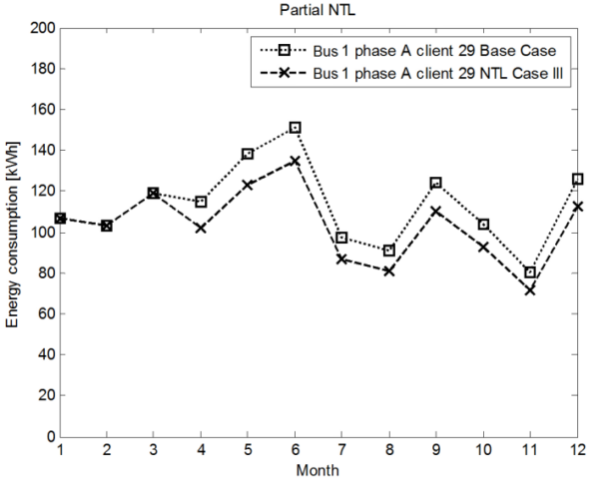
\includegraphics[scale=0.33]{decrease-partial.png}
			\caption{Čiastočné zníženie spotreby elektrickej energie~\cite{Trevizan2015}.}
			\label{fig:decrease-partial}
		\end{center}
	\end{minipage}
  \centering
  \begin{minipage}{0.45\textwidth}
    \begin{center}
      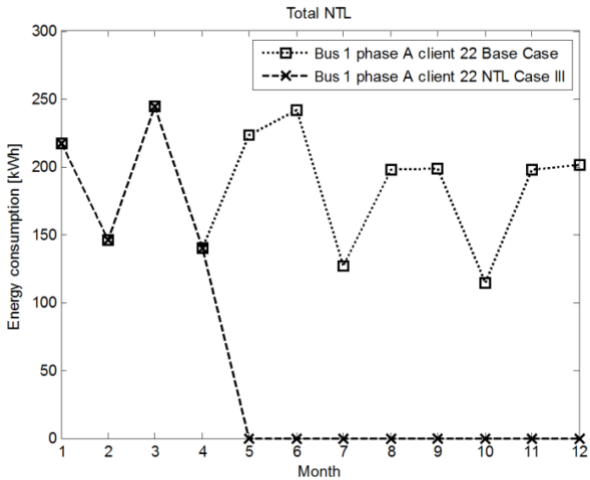
\includegraphics[scale=0.33]{decrease-total.png}
			\caption{Úplné zníženie spotreby elektrickej energie~\cite{Trevizan2015}.}
			\label{fig:decrease-total}
    \end{center}
  \end{minipage}\hfill

\end{figure}

%-------------------------------------------------------------------------------
%   Evaluation metrics
%-------------------------------------------------------------------------------

\subsection{Vyhodnocovacie metriky}


\subsubsection{Techniky detekcie anomálií}
Detegovať anomálie rôznych typov môžeme niekoľkými spôsobmi, čo závisí aj od
samotných dát. Ich úplnosť, množstvo a~oblasť, v~ktorej boli zozbierané sú
kritické pre správny výber techniky, pomocou ktorej budú identifikované anomálie.
Nás budú zaujímať najmä detekcie anomálií v~časových radoch. Popísané metódy
sú najmä z~oblasti strojového učenia a~dátovej analýzy, ale pre úplnosť sú
spomenuté aj iné používané metódy.

\paragraph{Klasifikácia}
Pomocou naučeného modelu, nazývaného aj klasifikátor, sú rozoznávané triedy
jednotlivých inštancií. Pri detekcii anomálneho správania, klasifikátor rozlišuje
iba medzi dvoma triedami, triedou normálnych dát a~anomálií. Vzhľadom na to, že
na natrénovanie klasifikátora sú potrebné označené dáta, ide o~učenie s~učiteľom.
Na implementovanie klasifikátora môžeme použiť techniky založené na rôznych
typoch neurónových sietí, Bayesovych sieťach, pravidlových systémoch či
SVM~\cite{Chandola2009,Tan2005}.

\paragraph{Analýza najbližšieho suseda}
Metóda určí na základe vzdialenosti alebo podobnosti medzi dátovými inštanciami,
či sa jedná o~normálnu inštanciu alebo anomáliu. To je vypočítané pomocou
vzdialeností medzi testovanou inštanciou a~všetkými bodmi, alebo iba \textit{k}
najbližšími bodmi. Pri viacrozmerných dátach je vzdialenosť určovaná pre
každú dimenziu zvlášť. Metóda je založená na predpoklade, že zatiaľ čo normálne
inštancie sa nachádzajú pri sebe a~sú husto usporiadané, anomálie sú vzdialenejšie,
prípadne na okraji vzniknutých oblastí. Aplikácia je možná pomocou techník založených
na relatívnej hustote alebo vzdialenosti najbližších \textit{k} susedných
inštancií~\cite{Chandola2009,Tan2005}.

\paragraph{Klastrovanie}
Jedná sa o~učenie bez učiteľa, keďže klastre inštancií sú vytvorené na základe
ich vzdialenosti či podobnosti. Techniky ďalej delíme do kategórií na základe
predpokladu o~dátových inštanciách~\cite{Chandola2009,Tan2005}.

Prvá kategória používa klastrovacie algoritmy ako DBSCAN alebo ROCK
a~vychádza z~predpokladu, že normálne inštancie patria do klastra, zatiaľ čo
anomálne nepatria do žiadneho. Keďže sa jedná o~klastrovacie algoritmy, nevýhodou
môže byť neoptimálne použitie pri detekcií anomálií~\cite{Chandola2009}.

Druhá kategória používa neurónové siete (konkrétne SOM) alebo algoritmus k-means.
Vychádza z~predpokladu, že normálne inštancie ležia v~blízkosti najbližšieho
centroidu, anomálne inštancie sú od neho vzdialené~\cite{Chandola2009}.

Posledná kategória pracuje s~predpokladom, že normálne inštancie sú súčasťou
veľkých a~hustých klastrov, na druhej strane anomálie patria do malých a~riedkych
klastrov. Používanými algoritmami sú napr. CBLOF (\textit{angl. Cluster-Based Local Outlier Factor}
) alebo \textit{k-d} stromy. V~princípe algoritmy najskôr vytvárajú klastre
a~až potom určujú, na základe ich hustoty, či sa jedná o~normálne klastre alebo
anomálie. Klaster je vytvorený iba v~prípade, že inštancia sa nachádza mimo
preddefinovaného rádiusu od centra daného klastra~\cite{Salvador2005}.


\newpage
\section{Rozpracovanie problému}
Pomocou metód strojového učenia a~dátovej analitiky sa zameriame na identifikáciu
anomálií v~oblasti distribučných spoločností. Na základe dát, ktoré máme
k~dispozícií zvolíme vhodnú metódu detekcie anomálií. Keďže dáta sú z~domény
distribúcie elektrickej energie, ich označenie by bolo finančne aj časovo
náročné. Rovnako aj spätná väzba pri identifikácií anomálií je časovo náročná
a~jej spracovanie môže trvať niekoľko týždňov až mesiacov.

Zameriavať sa budeme najmä na identifikáciu anomálií v~časových radoch, čo spadá
pod skupinové a~kontextové typy anomálií. Úlohou bude taktiež identifikovať
výhody a~nevýhody uplatnenia jednotlivých prístupov k~identifikácií. Zároveň
vzniká potreba nájsť najvhodnejšie techniky detekcií anomálií pre dáta zbierané
z~distribučných sietí pomocou inteligentných meračov. Najmä z~dôvodu, že každá
doména, v~ktorej je potrebné identifikovať anomálie sa vyznačuje špecifickými
potrebami na použitý model.


%-------------------------------------------------------------------------------
%   Chapter 8 - Bibliography
%-------------------------------------------------------------------------------

\newpage
\bibliographystyle{iso-690/slovakiso}
\bibliography{bibliography}

\end{document}

% \subsubsection{Nájdenie anomálií}
% \paragraph{Klasifikácia}
% \paragraph{Identifikácia najbližším susedom}
% \paragraph{Identifikácia zhlukovaním}
% \paragraph{Grafová analýza}
% \paragraph{Štatistické metódy}
% \paragraph{Hybridné prístupy}
% \paragraph{Spektrálna analýza}
